%!TEX root = ./m_main.tex


\chapter{Введение}

\section{О задаче восстановления и сохранения дерева процессов}
 
Основная задача, которая изучается в данной работе, называется “сохранение и восстановление состояния дерева Linux процессов”. Как мы видим, задача состоит из двух частей: сохранение и восстановление.
 
Сохранение состояния одного процесса включает в себя сохранение состояния всех ресурсов из которых состоит процесс, а также
сохранение состояния окружения, в котором исполняется процесс. Из каких ресурсов состоит типичный Linux процесс? Это 
регионы виртуальной памяти, открытые файлы, сокеты, устройства, идентификатор процесса, его сессия, группа, 
идентификатор текущего пользователя и так далее. Что входит в окружение процесса? Это пространства имен процесса 
(namespaces), контрольные группы (cgroups) и другое плюс их настройки. Стоит заметить, что при сохранении состояния 
процесса копии открытых им файлов не создаются. Это связано с тем, что файлы и так постоянно хранятся в ФС 
(файловой системе), а их копии могут занимать очень много места.

Что понимается под восстановлением состояния одного процесса? Это создание всех ресурсов процесса и всех объектов из его 
окружения, существовавших в момент сохранения, а также восстановление их состояния таким, каким оно было в момент 
сохранения. Важно, что после восстановления потоки процесса не должны заметить никакого изменения в поведении 
системных вызовов и своих машинных инструкций. То есть исполнение процесса должно продолжиться так, как если бы он не 
подвергался операциям сохранения и восстановления своего состояния. Внешние наблюдатели, то есть другие процессы в 
системе, тоже должны увидеть этот процесс максимально похожим на исходный сохраненный.

Выше были описаны задачи восстановления и сохранения одного процесса, но на практике нередки случаи, когда приложение состоит из нескольких процессов, имеющих общего родителя 
(child-parent relation). Каждый ребенок родителя может породить новые процессы приложения, а те в свою очередь другие 
процессы. В итоге, Linux приложения обычно представляют из себя дерево процессов, связанных отношением 
родитель-потомок. Кроме того, такая важная в современных облачных технологиях сущность как Linux контейнер, также 
представляет из себя дерево процессов с корнем, являющимся init процессом всего контейнера. Задача восстановления и 
сохранения дерева процессов требует, помимо состояний каждого из процессов в отдельности, поддерживать ещё и 
взаимоотношения между этими процессами, разделяемые ресурсы и другие особенности деревьев процессов в Linux.

\section{Актуальность задачи сохранения/восстановления}

\subsection{Живая миграция}

Живая миграция это перенос работающего приложения с одного узла кластера на другой, выполняемый незаметно для их пользователя. 
Живую миграцию можно выполнить с помощью сохранения и восстановления процессов приложения. Для этого нужно выполнить сохранение 
состояния процессов в файлы ФС на исходном узле кластера, скопировать файлы на целевой узел кластера, выполнить восстановление 
процессов из файлов на целевом узле. Если все эти операции выполняются за незаметное для пользователя время, то миграция является “живой”.
 
\subsection{Обновление ядра без остановки программ}
 
Для ядра Linux регулярно выходят обновления безопасности. При обновлении ядра нередко требуется его перезапуск и 
остановка всех процессов, работающих в ОС. Если процессы достаточно большие, например, БД занимающие 100~Гб 
оперативной памяти, то при пропускной способности чтения с диска в 100~Мб/с понадобится 1000~с = 15~мин, чтобы 
приложения считали свои данные с диска и восстановили свою работу после перезапуска. 15 минут это очень длительная 
задержка, которой можно избежать при использовании технологии сохранения и восстановления процессов без копирования их 
памяти. Для этого надо сохранить состояние приложений в оперативной памяти (без копирования страниц памяти приложений  \cite{url:lwn-kexec-persist-mem}), выполнить перезагрузку ядра, выполнить восстановление приложений без 
копирования их памяти.
 
\subsection{Отложенная отладка}
 
Благодаря технологии сохранения и восстановления процессов мы можем получить “живую” копию приложения для отладки на 
компьютере разработчика. Без данной технологии мы бы могли анализировать только дамп приложения - статичный снимок его 
состояния, полученный в определенный момент времени.
 
\subsection{Снимки приложений}
 
Технология сохранения и восстановления процессов позволяет создавать снимки состояний приложения в разные моменты времени и переключаться между ними. 
 
\subsection{Ускорение запуска программ}
 
Некоторые приложения выполняют большой объем работы при своем старте. Технология сохранения и восстановления процессов позволяет сохранить состояние приложения после завершения его инициализации. Вместо запуска приложения выполняется его восстановление в уже проинициализированном состоянии.

\section{Системная утилита \texttt{criu}}

Существует несколько программных решений задачи сохранения и восстановления процессов. В данной работе мы сосредоточимся на утилите \texttt{criu} \cite{url:criu}, обладающей следующими преимуществами перед другими проектами:

\begin{itemize}
	\item Работает в пространстве пользователя
	\item Не требует подмены динамических библиотек для отслеживания поведения процессов, в отличие от проекта DMTCP \cite{url:dmtcp}
	\item Не требует внесения тяжеловесных модификаций в ядро ОС, в отличие от проектов OpenVZ~\cite{url:openvz} и BLCR~\cite{url:blcr}
	\item Активно разрабатывается и поддерживается
\end{itemize}

Задача сохранения процесса решается в \texttt{criu} с помощью остановки целевого дерева процессов и вычитывания информации о нём с помощью интерфейсов, предоставляемым операционной системой: виртуальная система \texttt{/proc} (информация о процессе из вне), системные вызовы и чтение памяти (изнутри самого процесса). В проекта DMTCP, к примеру, используются обёртки над некоторыми функциями \texttt{glibc}, тем самым информация о процессе в том числе собирается в течение жизни процесса~\footnote{Конкретный момент времени исполнения тех или иных системных вызовов не сохраняется, поэтому по сути данный подход не добавляет никакой дополнительной полезной информации.}.

На этапе сохранения процесса программа производит анализ корректного, с точки зрения ОС, дерева процессов, создавая его снимок. Но дело в том, что снимок дерева говорит нам лишь о некотором закреплённом состоянии этого дерева и он не содержит информации о том, как именно оно пришло в это состояние. С течение времени дерево процессов эволюционирует:

\begin{itemize}
	\item Открывает файлы, сокеты, каналы и пр
	\item Модифицирует виртуальное пространство удаляя и добавляя области (\texttt{mmap})
	\item Создаёт дочерние процессы
	\item Переходит из группы в группу
	\item Переходит из одного пространства имён в другое (namespaces)
	\item Переходит в новую сессию
	\item ...
\end{itemize}

Каждая из операций переводит процесс из одного состояние в другое и если мы представим себе граф состояний и переходов
между ними, то легко увидим, что такой граф обладает нетривиальной структурой:

\begin{itemize}
	\item Между двумя состояниями дерева может быть много путей: файлы можно открывать в разной последовательности; для того, чтобы 2 процесса, родитель и ребёнок, ссылались на один и тот же файл по одному и тому же файловому дескриптору, можно открыть файл родителем, после чего совершить \texttt{fork} ребёнка, а можно сначала совершить \texttt{fork}, а потом передать файловый дескриптор используя сокеты домена Unix.

	\item Существуют состояния дерева, между которыми нет пути: процесс, находящийся в определённом пространстве идентификаторов процесса (pid-namespace) не может стать процессом из другого пространства (и наоборот); Процесс лидер сессии (session leader) не может перестать быть им
\end{itemize}

Таким образом восстановление дерева процессов должно быть реализовано так, что в каждый момент времени наше текущее состояние дерева процессов ещё имеет возможность добраться до состояния целевого, переходя по рёбрам --- системным вызовам (и другим операциям, изменяющим состояние процесса). Необходимость поддерживать это свойство во время восстановления и делает задачу сложной: мы не можем просто взять и для каждого ресурса процесса написать независимую от текущего состояния этого процесса (и дерева процессов) функцию, которая бы просто выполняла восстановление этого ресурса~\footnote{Для некоторых ресурсов процесса это возможно: состояния регистров потоков процесса и др.}.

\section{Проблемы текущего подхода \texttt{criu} к восстановлению}

\texttt{Criu} хорошо справляется с задачей восстановления большого количество процессов с различными ресурсами, но
текущий подход к процедуре восстановления --- это некоторая зафиксированная последовательность из большого количества шагов. Проверка файлов снимка дерева, инициализация \texttt{vdso}, частичное считывание информации из образа и инициализация различных структур, которые используются при восстановлении. В том числе тут происходит инициализация информации о процессах-помошниках, которые нужны, например, для того, чтобы верно восстановить сессии процессов, которые когда-то были <<усыновлены>> процессом \texttt{init}~\footnote{Такое происходит, когда процесс-родитель завершается раньше ребёнка}. Далее начинается процедура восстановления: происходит восстановление корневого процесса и пространств имён для него (которые далее наследуются), создание дерева процессов (fork), и т.д. Такая цепочка действий чётко зафиксирована в коде \texttt{criu}.

Цепочка чётко отсортированных шагов выражает индивидуальных подход к восстановлению каждого из ресурсов. Это приводит к следующим проблемам:

\begin{itemize}
	\item Код для восстановления каждого типа ресурсов нужно добавить в последовательность действий по восстановлению всего дерева так, чтобы его логика согласовывалась со всей остальной логикой, которой очень много ведь последовательность действий очень длинная
	\item Любые нетривиальные зависимости между ресурсами требуют добавления дополнительного кода в цепочку действий, обрабатывающего эту нетривиальность
	\item Фиксированная цепочка действий может являться потенциальной причиной меньшего множества возможных к восстановлению процессов, чем могло бы быть (вспомним про метафору графа состояний дерева процессов, описанную выше)
	\item Отсутствие чёткого понимания того, какие конфигурации ресурсов дерева процессов \texttt{criu} 100 процентно поддерживает
\end{itemize}

Сложность и отсутствие гибкости цепочки действий приводит к тому, что восстановление определённых ресурсов и взаимосвязей между ними трудно реализуемо. Рассмотрим в качестве примера группы процессов в дереве процессов, изображённом на рисунке~\ref{chap1:fig:groupstree}.

\begin{figure}[ht!]
	\centering
	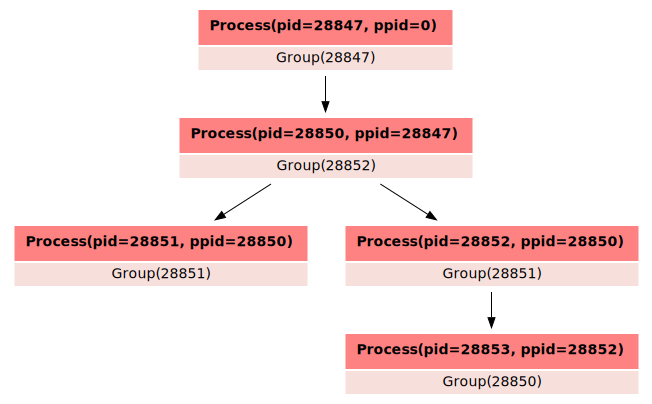
\includegraphics[scale=0.5]{fig/groups-pstree.pdf}
	% \scalebox{.5}{\import{fig/}{groups-pstree.pdf_tex}}
\caption{Дерево процессов}
\label{chap1:fig:groupstree}
\end{figure}

В Linux, группа с идентификатором $28852$, может быть создана только в процессе с идентификатором (pid) равным $28852$.
Но как мы видем из рисунка~\ref{chap1:fig:groupstree}, процесс $28852$ в целевом дереве находится в другой группе, а именно в $28851$. На таком дереве процессов \texttt{criu} завершается с ошибкой о том, что не может присвоить процессу $28850$ группу $28852$. Это происходит из-за того, что на момент исполнения системного вызова установки группы, группы $28852$ ещё (или уже) вовсе не существует. Данное дерево процессов является нетривиальным, так как его восстановление требует того, чтобы во время жизни процесс $28852$ побывал сначала в одной группе ($28852$), а потом оказался в другой.

\section{Возможные подходы к решению проблемы восстановления}
\label{chap1:sec:approaches}

Каким образом можно избежать проблем, описанных в предыдущем разделе? На данный момент, методов, которые решают проблему восстановления дерева процессов, качественнее чем \texttt{criu}, нет~\footnote{В рамках ограничений пользовательского приложения}. Но в предыдущих работах, касающихся этой проблемы, был озвучен общий подход: разделение процедуры восстановления на несколько этапов (см. рис~\ref{chap1:fig:stages}).

\begin{figure}[ht!]
\centering
\begin{small}
\minibox[frame]{Файлы образы\\дерева процессов} 
$\xRightarrow{\text{анализ}}$ 
\minibox[frame]{Промежуточное\\представление 1}  
$\xRightarrow{\text{анализ}}$ 
\minibox[frame]{Промежуточное\\представление 1}  
$\xRightarrow{\text{...}}$ 
\minibox[frame]{Команды для\\восстановления}  
\end{small}
\caption{Разделение на этапы}
\label{chap1:fig:stages}
\end{figure}

Каждый этап (количество этапов не специфицируется) производит анализ результатов предыдущего шага. Всё начинается с анализа файлов-образов процесса, считываемых с диска. Промежуточное представление --- это представленные определённым и удобным для некоторых целей, данные. Тут можно провести аналогию с компиляторами, где промежуточными представлениями выступают структуры, такие как абстрактное синтаксическое дерево, single static assignment form и др. Они служат вспомогательными структурами, которые помогают выполнять те или иные операции эффективнее и проще.

Конечным же продуктом череды промежуточных представлений является набор команд. Этот набор команд предполагает, что он может быть исполнен процессом-интерпретатором так, что итогом исполнения является целевое дерево процессов (восстановленное).

Вопросы, который ставит данных подход:

\begin{itemize}
	\item Каковы должны быть промежуточные представления?
	\item Какой вид имеет финальный список команд?
\end{itemize}


Такой подход предполагает разделение разделение восстановления на генерацию и интерпретацию команд: генератор и интерпретатор. А значит, у нас появляется свобода выбора: насколько сложным делать генератор и интерпретатор. Ясно, что интерпретатору придётся делать системные вызовы~\footnote{Именно с помощью системных вызовов производится большая часть изменений состояния процесса} для приведения дерева процессов в нужное состояние. Это значит, что наиболее простой с точки зрения интерпретатора набор команд --- это набор системных вызовов, которые нужно последовательно исполнить. В такой ситуации генератор будет максимально сложным. Таким образом параметром данного подхода в том числе является компромисс между сложностью интерпретатора и генератора.

Одним из возможных промежуточных представлений как раз является граф ресурсов. Каждый ресурс, такой как процесс, поток, сессия, файловый дескриптор, OFD, регион памяти и так далее, является в этом графе вершиной с атрибутами, такими как PID, путь в ФС, id, размер и так далее. Ребра в таком графе направленные и представляют собой отношения между ресурсами.

Подход с разделением восстановления на многоступенчатый генератор и интерпретатор позволяет сделать процесс восстановления более гибким и простым:
\begin{itemize}
	\item Генератор можно реализовывать независимо от платформы, т.к. системных вызовов он не выполняет
	\item Генеративный подход имеет больший потенциал, чем зафиксированная последовательность действий, т.к. может генерировать абсолютно разные последовательности команд (это зависит от промежуточных представлений и т.д.)
\end{itemize}

\section{Задачи и требования}

Задача, которая была поставлена при выполнении данной работы, заключается в следующем:

\begin{itemize}
	\item Предложить промежуточные представления для генератора и компромисс между сложностью генератора и интерпретатора
	\item Разработать генератор команд для задачи восстановления дерева процессов в рамках подхода генератор-интерпретатор, описанного в разделе~\ref{chap1:sec:approaches}
\end{itemize}

Общими требованиями к итоговому решению являются:
\begin{itemize}
	\item Поддержка как можно большего числа ресурсов процессов в Linux
	\item Возможность эффективной реализации предлагаемых алгоритмов
\end{itemize}


\section{Содержание данной работы}

В данной части мы вкратце описали проблемы текущих подходов к восстановлению дерева процессов и возможные подходы к решению этих проблем, а так же сформулировали задачи. В части~2 подробно раскрывается конкретное промежуточное представление и подход к генерации команд, предлагаемых в данной работе. Этот подход основан на модели жизнедеятельности (обмена ресурсами) процессов в Linux и графе абстрактных действий, которые процессы совершают, чтобы этими ресурсами обмениваться, создавать их и уничтожать. В последней части, подводятся итоги и описываются дальнейшие планы на развитие подхода, предлагаемого в этой работе.
